% Based on LLNCS macro package for Springer Computer Science proceedings;
% Version 2.20 of 2017/10/04
\documentclass[runningheads,a4]{llncs}
\usepackage{pre}

\begin{document}

\maketitle

\section{Business Case}
\label{sec:business}
Urban mobility is rapidly evolving, not only due to the increased awareness with
environmental issues, but because of the huge impact digitalization has on the
traditional ways people are able to use transportation systems.

The idea behind \ac{MaaS} is analogous to that of \ac{SaaS}, a term popularized
by Cloud technology: people use the transport network they see better fits their
needs while doing so in a flexible and easy fashion, also enabling the inclusion
of innovative alternatives for personal transportation like rental bike,
scooters, motorcycles, and the likes.

The main challenge arises when it comes to seamlessly integrating all of these
services together without the hassles that come with the need of multiple
ticketing mechanisms or devices, be it through the usage of physical cards or
different mobile applications, proving card/device and fare payment management
arduous tasks.

\subsection{Business Description}
\label{sec:business.description}
The \ac{MaaS} platform must be capable of incorporating several transportation
services with ease, enabling further operation adherence in the future, as well
as providing the customer a satisfying experience by removing the need to manage
all of the little intricacies of using multiple different transportation
networks.

To that end, the goal is to model an event-driven system agnostic from the
transportation operator by implementing mechanisms for handling certain types of
"ways of consuming transportation". Take, for example, the myriad of ways public
transportation can be consumed: via pre-paid cards, for one-off trips, or using
a temporal tickets, where the price can be correlated to the amount of time
spent within the public transport's boundaries.

Besides public transportation, a rise in private transportation providers
popularity requires attention. However, one can easily integrate with such
providers with a similar approach by appropriately adapting to the ways such
providers offer transportation services.

\subsection{Business Value}
\label{sec:business.value}
By successfully achieving integration goals described previously, we must
establish an interoperable service bus through which the various entities of the
system can interact and communicate with, effectively assembling a network of
transportation operators. The ease of integration brings more transportation
operators into the system, which increases the appeal for a wider range of
customers to enroll in the platform.

From the transportation operators' perspective, a platform that gathers the
users of several other operators has the potential of bringing new customers and
increase revenue with almost no effort.


\section{Entities}
\label{sec:entities}
The MaaS platform is comprised of a few different entities, among which are the
platform’s customers, or clients, capable of using the means of transportation
offered by the transportation service providers, or operators, another set of
entities in the system, that the platform integrates with.

Transportation service providers, as the designation entails, provide a series
of heterogeneous transportation services for the customer to consume. As it
stands, the platform provides three different types of services:
\begin{enumerate*}[label=(\arabic*)]
  \item check-in/check-out, which resembles an ephemeral one-time on-demand
        pre-paid model of using transportation,
  \item flat fare, for one-shot temporally independant trips or even similar to
        a subscription-like consumption model (e.g. monthly pass), and
  \item operator-defined, where the operator might possess complex logic for
        computing the fare of a trip, hence calculating it \emph{in-premises}
        and providing the value after the fact (e.g uber, taxify).
\end{enumerate*}

To incorporate the aforementioned entities into the system, we essentially
require a set of both internal and external services in order to enroll
transportation service providers, their respective products/services, and to
enroll users/customers.

Essentially, a human management corp is required for assessing operator
registration requests as part of a semi-automatic process for doing so, as well
as for revising subsequent product/service registration requests, again, on the
operator's behalf.

To enroll transportation service providers, we must integrate with a few
external fiscal information and postal address services to perform proper
validation and information gathering.

With respect to the customers, the system also encompasses a virtual payment
service provider (outside the scope of the actual implementation) in order for
the customers to perform payment orders emitted by the system as transportation
services are provided.


\section{Functional Specification}
\label{sec:function}
The platform is comprised of a series of business processes and services that
enable correct functionality of the system. Customer and transportation
operators enrolment is made available through business processes. When
enrolling, transportation operators provide their information and that
information is verified by the system with the help of a human (\ac{MaaS}
management corp). When the process completes successfully, the system creates a
channel through which the operator can send events related to the user trips.
Our system provides a simple contract for those events. 

When the users register in the \ac{MaaS} platform, a token is generated and
associated to that user.  The operator/validator sends events related to a user
and the platform is responsible for handling the payment orders for that user
and to adequately distribute the revenue across the operators. The payment order
is ran by an account management service that attempts to make a funds request to
a payment service provider. If the payment is rejected, the user is blacklisted
and all the operators are notified. Otherwise, the system registers a trip for
the user. Based on the trips made, the user gets rewarded with discounts that
can be percentage-based or flat.

\section{Business Processes}
\label{sec:processes}
In whole, we've designed three business processes: one for registering a
customer in the platform, illustrated in \Cref{fig:bpel.customer}, and two other
processes for registering a transportation service provider and the
products/services it provides, respectively shown in
\Cref{fig:bpm.operator,fig:bpm.service}.

\begin{figure}
  \centering
  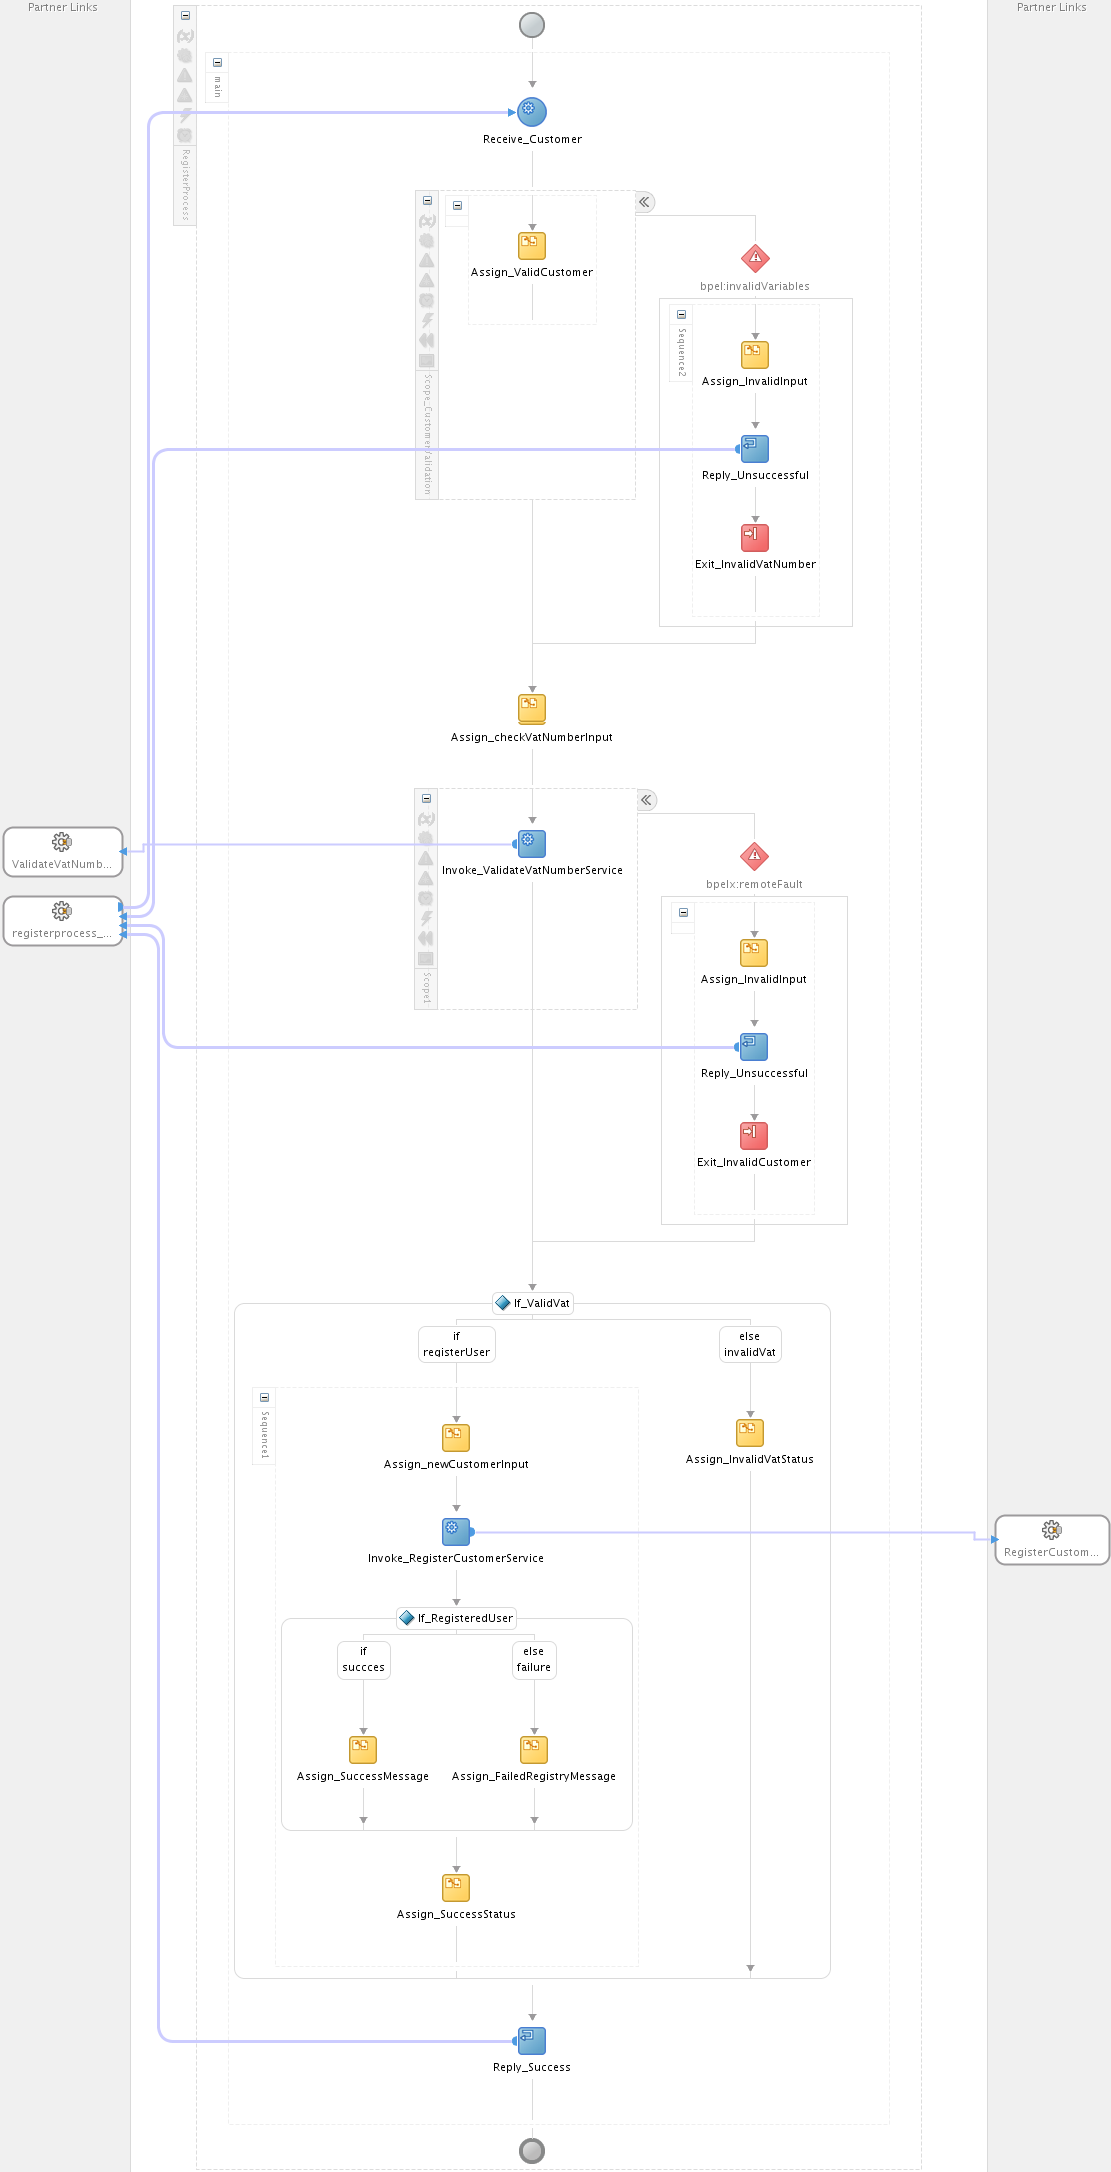
\includegraphics[height=\textheight]{img/bpel-customer.png}
  \caption{Business process for enrolling a transportation service provider}
  \label{fig:bpel.customer}
\end{figure}
\begin{sidewaysfigure}
  \centering
  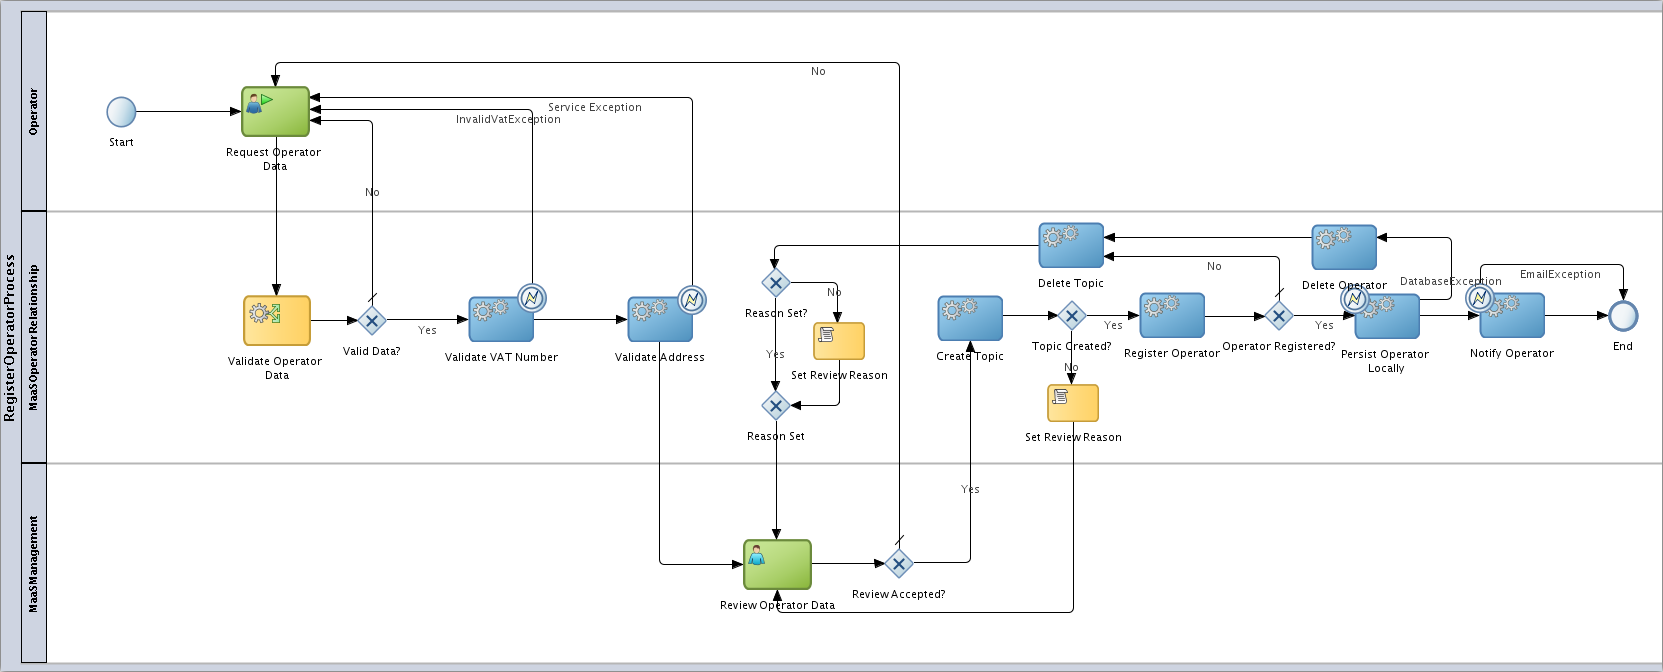
\includegraphics[width=\textwidth]{img/bpm-operator.png}
  \caption{Business process for enrolling a transportation service provider}
  \label{fig:bpm.operator}
\end{sidewaysfigure}
\begin{sidewaysfigure}
  \centering
  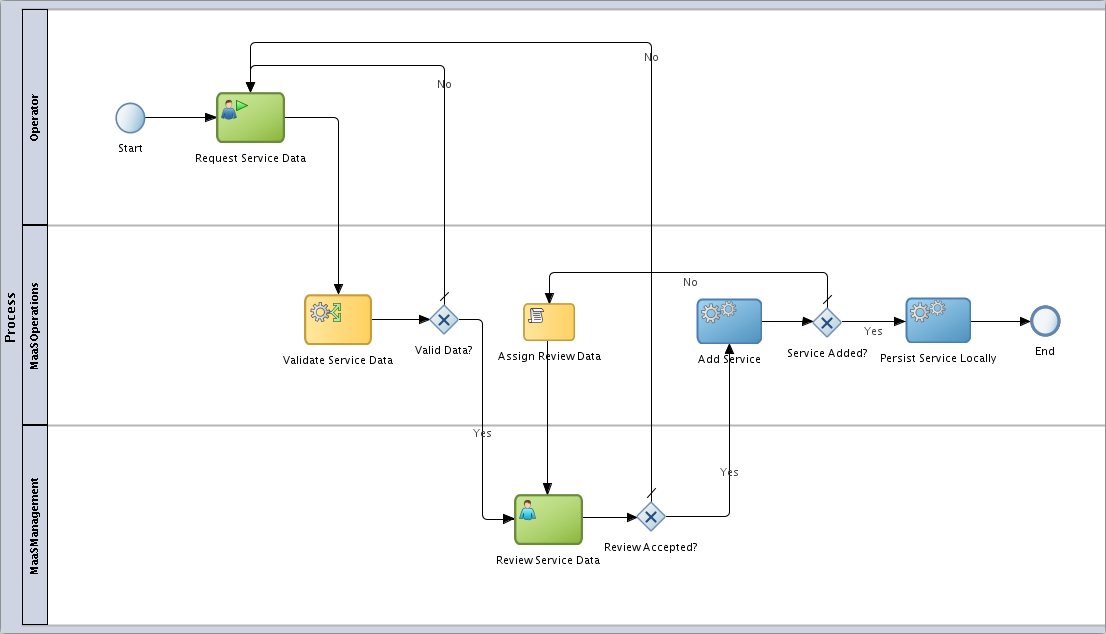
\includegraphics[width=\textwidth]{img/bpm-service.png}
  \caption{Business process for enrolling a transportation service provider's
    product/service}
  \label{fig:bpm.service}
\end{sidewaysfigure}


\section{Architecture}
\label{sec:architecture}
The system's composed of an assortment of micro-services deployed in a Cloud
environment (specifically, \ac{AWS}), and services generated from \ac{BPEL} and
\ac{BPMN} processes using the Oracle 11g \ac{SOA} Suite software. A visual
depiction can be seen in \Cref{fig:archimate.architecture}.

The cloud services are all written in different languages whilst the Oracle
software ones are pure Java.

\begin{figure}
  \centering
  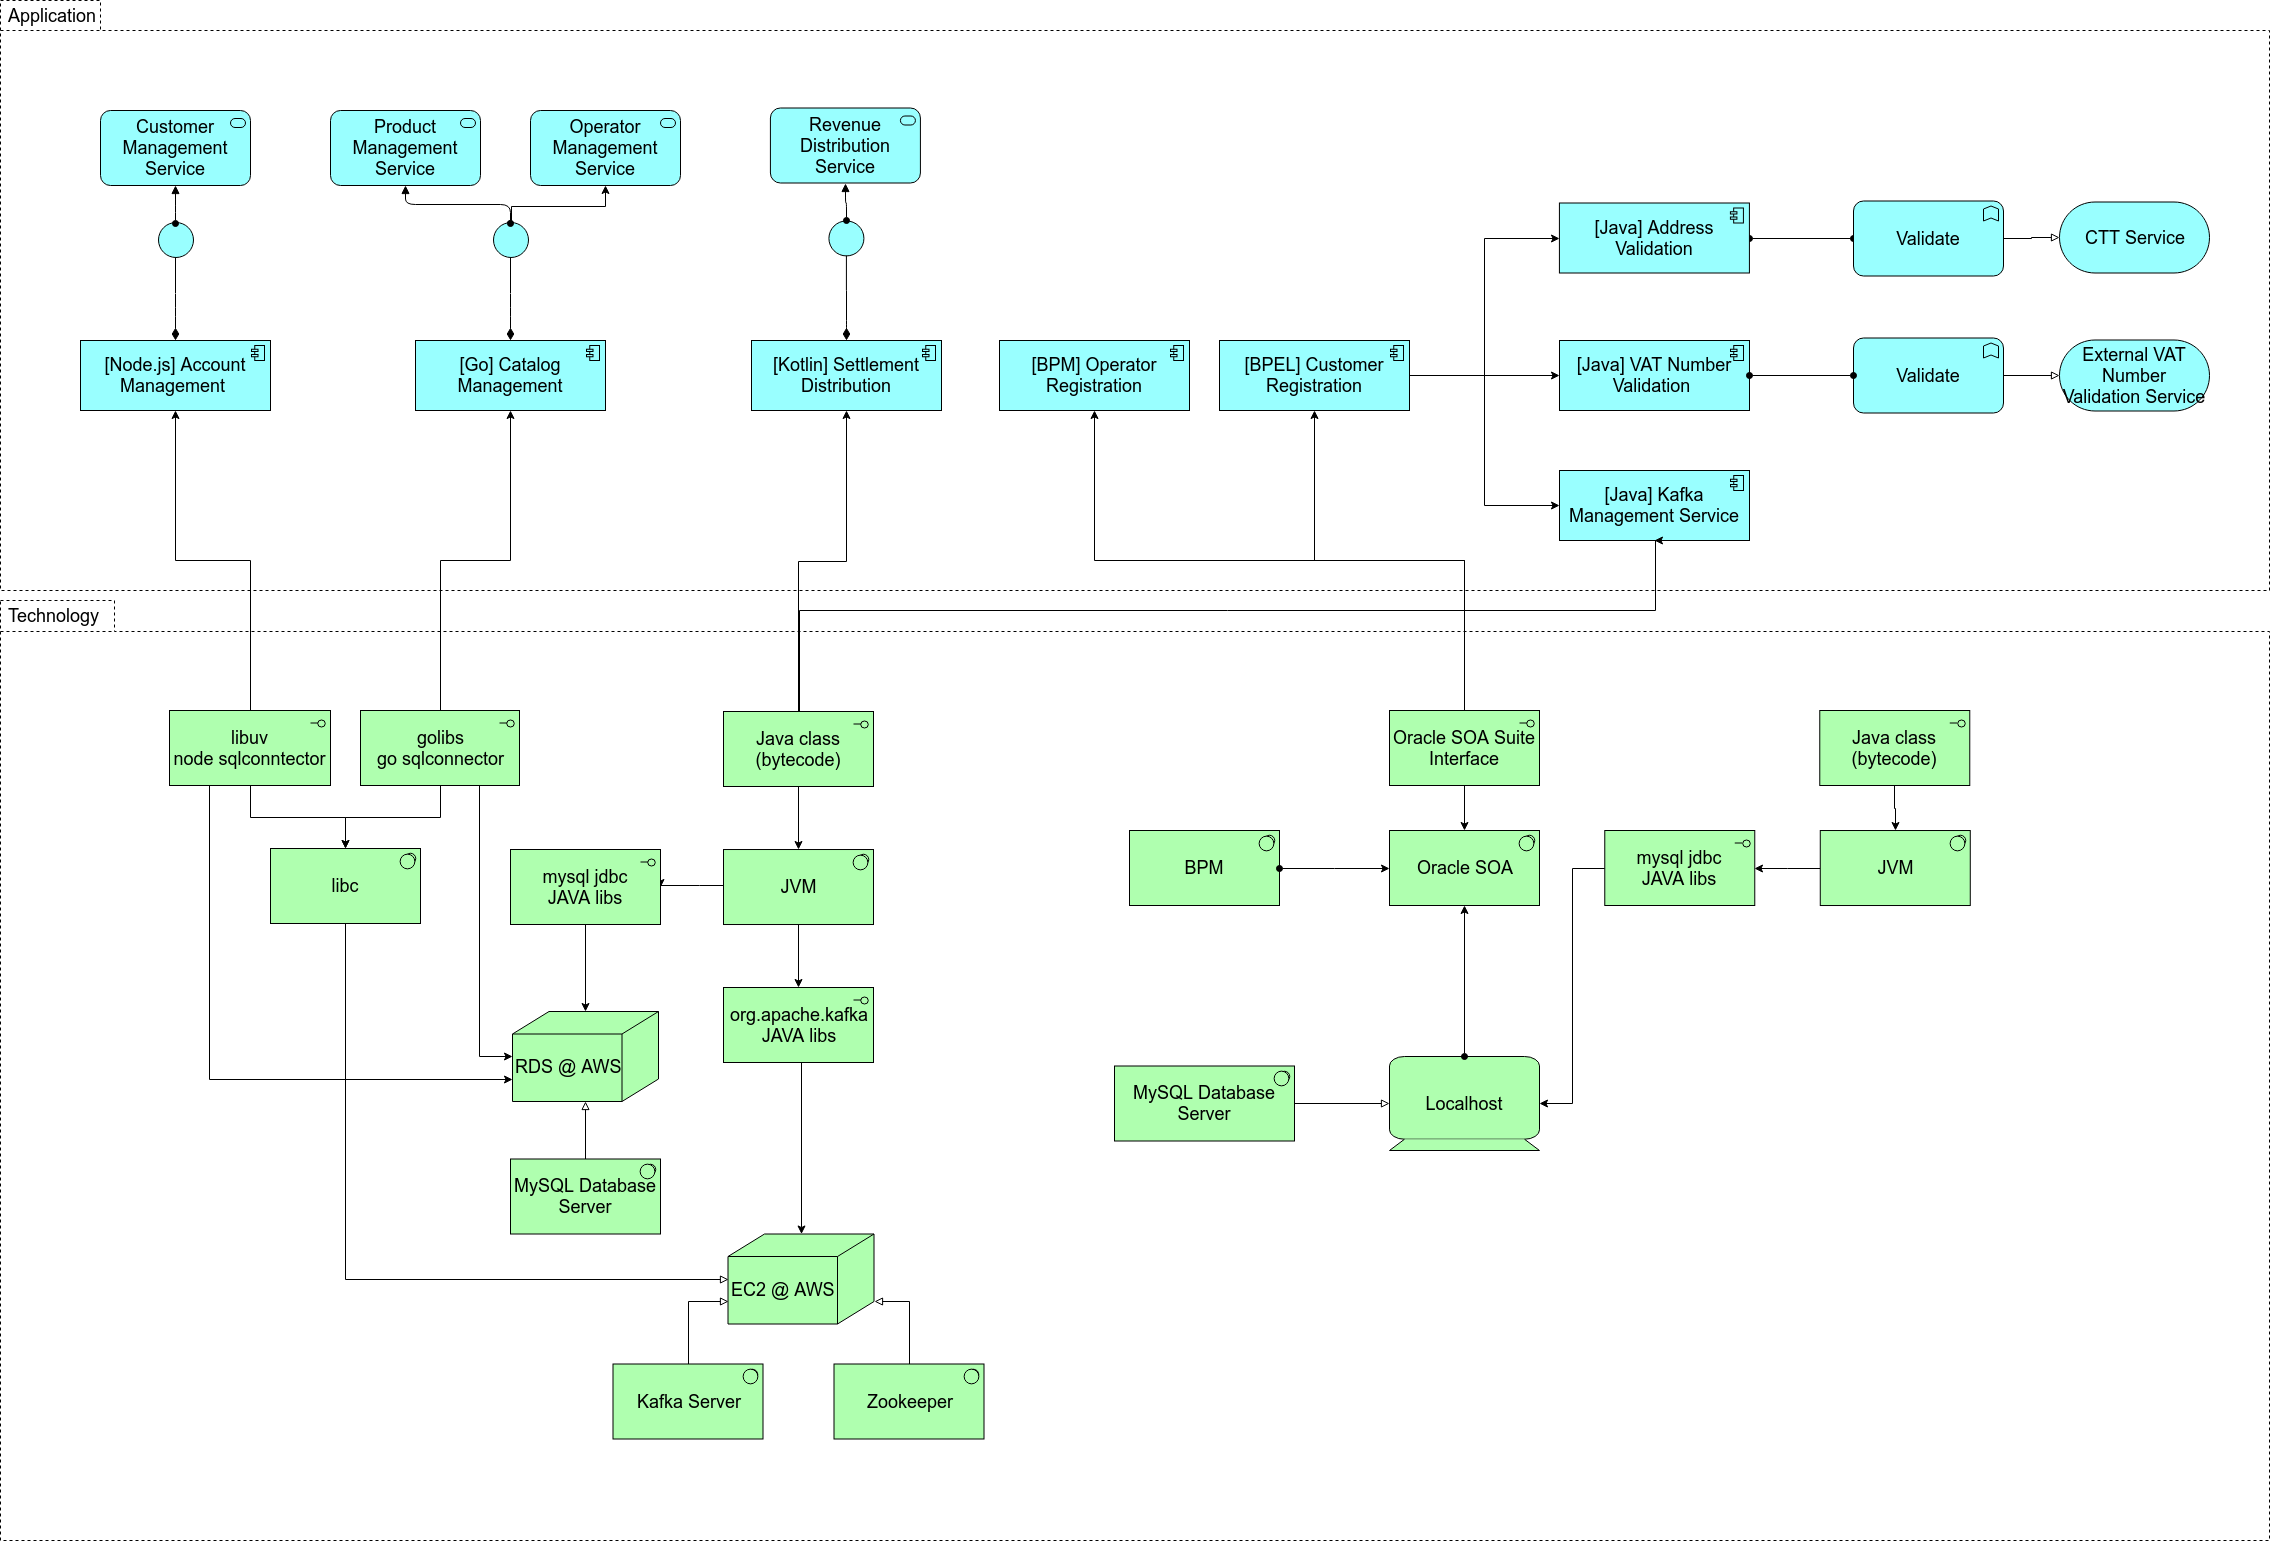
\includegraphics[width=\textwidth]{img/archimate-architecture.png}
  \caption{Archimate model of the system architecture}
  \label{fig:archimate.architecture}
\end{figure}


\newpage
\section{Services}
\label{sec:services}
As previously mentioned, the platform is composed of a series of services
crucial to the system's correct functionality. These come in the way of internal
services hosted in the cloud and the ones used by the business processes,
showcased in \Cref{fig:service-hierarchy}.

\subsection{Catalog Management}
\label{sec:services.cloud.catalog}
This service is tasked with keeping the set of products, their respective
prices, and usage rules for each of the transportation operators' products,
providing this information as a collection to the other services, or even the
customer, when required.

\subsection{Settlement Distribution}
\label{sec:services.cloud.settlement}
This service is responsible for registering trip events published by the user
and appropriately distributing the revenue across the operators, taking into
account several aspects that may influence the computation which can be service
dependant, such as the trip's duration.

\subsection{Account Management}
\label{sec:services.account}
This service handles customer related operations. It handles customer
registration alongside the \ac{BPEL} process showcased in
\Cref{fig:bpel.customer}, persisting pertinent user information; it manages the
user’s finances inside the system, issuing debit orders and blacklisting the
users whose balance prevents th\ac{JSON}em from using the integrated transportation
services. Furthermore, it is responsible for determining discount values for
customers using the platform.

\begin{figure}
  \centering
  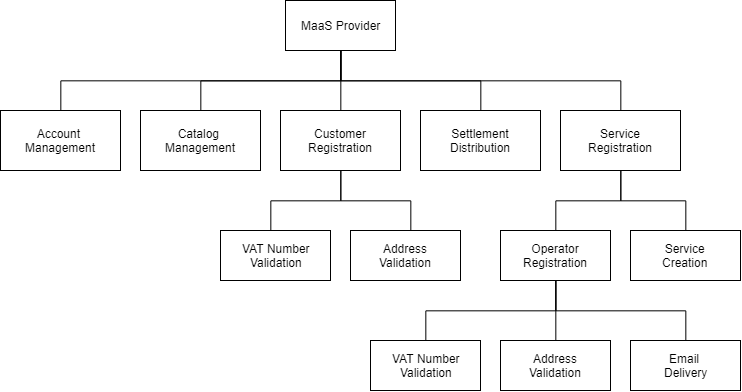
\includegraphics[width=\textwidth]{img/service-hierarchy.png}
  \caption{\acs{MaaS} platform service hierarchy}
  \label{fig:service-hierarchy}
\end{figure}


\section{Data Schemas}
\label{sec:schemas}
The following figures illustrate the data being persisted on the services
described in \Cref{sec:services}. As a sidenote, the business process persist
operator and service data much akin to how the Catalog Management service does,
as seen in \Cref{fig:sql.catalog-ws}.

Additionally, the Settlement Distribution service persists events that come into
the message broker (see \Cref{sec:kafka}) \emph{quasi-}literally, using an
\ac{ORM} framework, as it performs the required computation when they come in,
using them later to distribute the revenue among operators. As such, instead of
a relational database diagram, a \ac{UML} object diagram is presented (see
\Cref{fig:uml.settlement-ws}) to highlight similarities and relationships
between objects hidden by the \ac{ORM}.

\begin{figure}
  \centering
  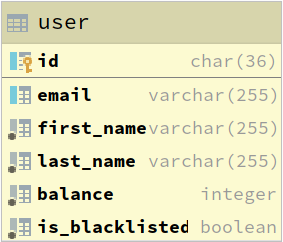
\includegraphics{img/sql-account-ws.png}
  \caption{Account Management service database schema}
  \label{fig:sql.account-ws}
\end{figure}
\begin{figure}
  \centering
  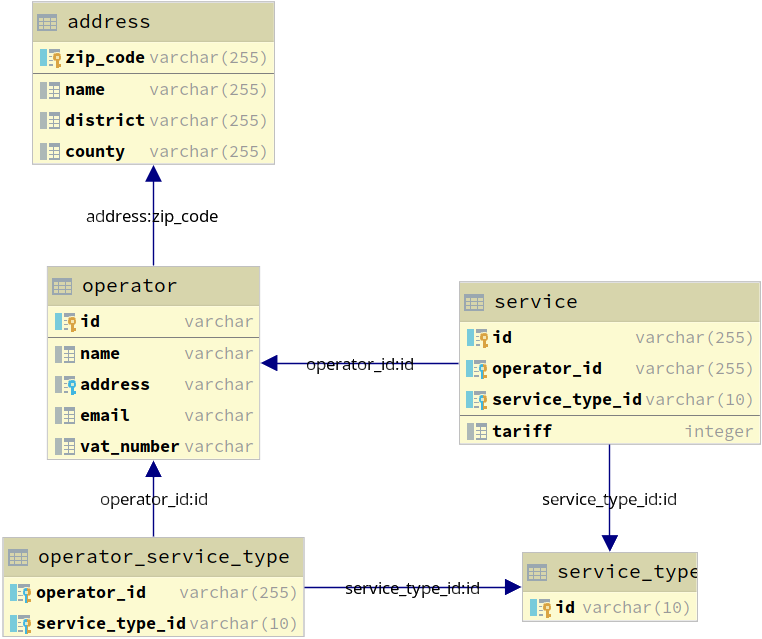
\includegraphics{img/sql-catalog-ws.png}
  \caption{Catalog Management service database schema}
  \label{fig:sql.catalog-ws}
\end{figure}
\begin{figure}
  \centering
  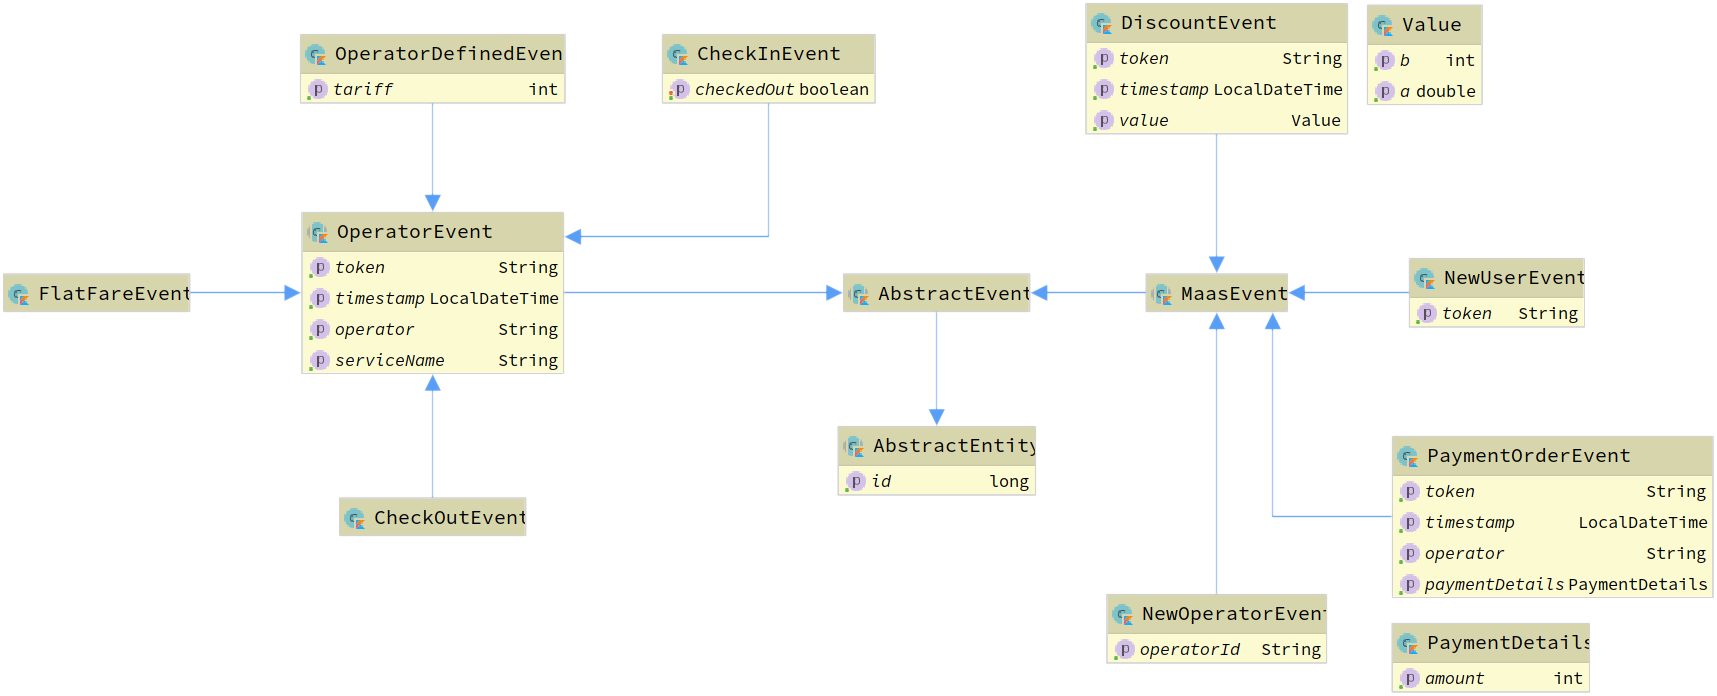
\includegraphics[width=\textwidth]{img/uml-settlement-ws.png}
  \caption{Settlement Distribution service \acs{UML} object diagram}
  \label{fig:uml.settlement-ws}
\end{figure}

\section{Kafka}
\label{sec:kafka}
In order for transportation service providers to integrate with the platform,
the system relies on a message broker in order to consume events emitted by
operators and function properly.

\subsection{Topics}
\label{sec:kafka.topics}
The message broker will have as many topics as there are operators that are
registered in the system, plus an additional topic for internal management. The
name of the topic for each operator is chosen by the \ac{MaaS} management
revisor during registration, which is returned to the operator when registration
goes through (see \Cref{fig:bpm.operator}).

For simplicity's sake, every topic only has a single partition and a replication
factor of 1 since there is only one broker.

\subsection{Events}
\label{sec:kafka.events}
Events are serialized as JavaScript objects, appropriately, in \ac{JSON}. The
following sections describe the events that arrive at the message broker, broken
into two categories:
\begin{enumerate*}[label=(\arabic*)]
  \item Operator events, which are the events that arrive at the operator
        specific topics, and
  \item \ac{MaaS} events, these being the internal events.
\end{enumerate*}

\subsubsection{Operator Events}
\label{sec:kafka.events.operator}
~\\~\\
The general schema for operator events is as follows:

\begin{itemize}[leftmargin=8em]
  \item[\texttt{type}] String - one of: \texttt{flat-fare},
    \texttt{check-in check-out}, \\\texttt{operator-defined}
  \item[\texttt{token}] UUIDv4 - user token
  \item[\texttt{service\_name}] String - Name of the service
  \item[\texttt{timestamp}] ISO 8601 UTC timestamp
  \item[\texttt{tariff}] Integer (optional, only in \texttt{operator-defined})
\end{itemize}

An example can be seen in \Cref{lst:json.events.operator}.

\subsubsection{\acs{MaaS} Events}
\label{sec:kafka.events.maas}
Internal events are slightly more disparate from each other in terms of
structure.

The schema for a new user event is as follows:

\begin{itemize}[leftmargin=7em]
  \item[\texttt{type}] String - \texttt{new-user}
  \item[\texttt{user}] User object
\end{itemize}

\clearpage
The user object is described as follows:

\begin{itemize}[leftmargin=9em]
  \item[\texttt{id}] UUIDv4 - user token
  \item[\texttt{email}] String
  \item[\texttt{first\_name}] String
  \item[\texttt{last\_name}] String
\end{itemize}

An example can be seen in \Cref{lst:json.events.new-user}.


The schema for a new operator event is as follows:

\begin{itemize}[leftmargin=8em]
  \item[\texttt{type}] String - \texttt{new-operator}
  \item[\texttt{operator}] String - operator identifier, i.e., topic name
\end{itemize}

An example can be seen in \Cref{lst:json.events.new-operator}.


The schema for a payment order event is as follows:

\begin{itemize}[leftmargin=12em]
  \item[\texttt{type}] String - \texttt{payment-order}
  \item[\texttt{token}] UUIDv4 - user token
  \item[\texttt{payment-details}] Payment Details object 
\end{itemize}

The payment details object is described as follows:

\begin{itemize}[leftmargin=7em]
  \item[\texttt{amount}] Integer - amount user has to pay
\end{itemize}

An example can be seen in \Cref{lst:json.events.payment-order}.


The schema for a blacklist/whitelist events is as follows:

\begin{itemize}[leftmargin=7em]
  \item[\texttt{type}] String - \texttt{blacklist}/\texttt{whitelist}
  \item[\texttt{user}] UUIDv4 - user token
\end{itemize}

N.B.: Unlike the other events described in this section, this event isn't sent
to the internal \ac{MaaS} system topic. It is sent to the operator topics so
information about the blacklisted/whitelisted user can be propagated throughout
the respective operators' systems. An example can be seen in
\Cref{lst:json.events.blacklist}.


The schema for a discount event is as follows:

\begin{itemize}[leftmargin=7em]
  \item[\texttt{type}] String - \texttt{blacklist}/\texttt{whitelist}
  \item[\texttt{user}] UUIDv4 - user token
  \item[\texttt{value}] Value object
\end{itemize}

The value object is described as follows:

\begin{itemize}[leftmargin=7em]
  \item[\texttt{a}] Decimal - a ratio applied to the base value
  \item[\texttt{b}] Integer - flat discount
\end{itemize}

An example can be seen in \Cref{lst:json.events.discount}.




\begin{listing}[htbp]
  \inputminted{json}{src/operator.json} 
  \caption{General example of all operator events}
  \label{lst:json.events.operator}
\end{listing}

\begin{listing}[htbp]
  \inputminted{json}{src/new-user.json} 
  \caption{New user event example}
  \label{lst:json.events.new-user}
\end{listing}

\begin{listing}[htbp]
  \inputminted{json}{src/new-operator.json} 
  \caption{New operator event example}
  \label{lst:json.events.new-operator}
\end{listing}

\begin{listing}[htbp]
  \inputminted{json}{src/payment-order.json} 
  \caption{Payment order event example}
  \label{lst:json.events.payment-order}
\end{listing}

\begin{listing}[htbp]
  \inputminted{json}{src/blacklist.json} 
  \caption{Blacklist/Whitelist event example}
  \label{lst:json.events.blacklist}
\end{listing}

\begin{listing}[htbp]
  \inputminted{json}{src/discount.json} 
  \caption{Discount event example}
  \label{lst:json.events.discount}
\end{listing}


\begin{acronym}
  \acro{AWS}{Amazon Web Services}
  \acro{BPEL}{Business Process Execution Language}
  \acro{BPMN}{Business Process Model and Notation}
  \acro{JSON}{JavaScript Object Notation}
  \acro{MaaS}{Mobility as a Service}
  \acro{ML}{Metro de Lisboa}
  \acro{ORM}{Object-relational Mapping}
  \acro{SaaS}{Software as a Service}
  \acro{SOA}{Service Oriented Architecture}
  \acro{TTSL}{Transtejo \& Soflusa}
  \acro{UML}{Unified Modelling Language}
\end{acronym}
\end{document}
